\clearpage
\twocolumn[{%
\subsection{Benchmark design}
\label{app:rq09_benchmark_design}

\noindent\begin{minipage}[t]{0.485\textwidth}
\vspace{0pt}
\paragraph{Research Question.} \emph{Why do some multilingual benchmarks separate models cleanly under the SNR framework and others don't? Is it curation quality, task format, item length, or the answer space?}

\paragraph{Setup.} Seed-1904 runs of every cell. SNR is the mean pairwise distance over noise at the 1.7B reference. For each family, we take the median over its per-language tasks. We keep the benchmark families that clear the above-chance gate. We group the families by curation, source, task format, answer-option count and passage use, and we test the groups with a Kruskal-Wallis test.
\end{minipage}\hfill
\begin{minipage}[t]{0.485\textwidth}
\vspace{0pt}
\begin{rqfinding}
\textbf{1. With every benchmark in, the answer-option count orders the families by SNR, but no characteristic orders them by DA-size in both readings.} The six 2-option families have a median SNR of 1.91 against 0.75 for the eighteen 4-option ones (Kruskal-Wallis H = 11.32, p = 0.003, under 0.05 after a Bonferroni correction for the five axes, and Spearman $\rho$ = $-$0.65 with a 95 \% interval of $-$0.84 to $-$0.33). The five sharpest families are MultiBLiMP 2.39 (34 tasks), HellaSwag 2.29 (26), XStoryCloze 2.18 (8), Global PIQA non-parallel 2.06 (2) and XWinograd 1.77 (6), and the reformulated twins and the English-only benchmarks fill the lower half (0.56 to 1.09). (Figure~\ref{fig:app_rq09_benchmark_design}.)
\\
\\
\textbf{2. The benchmark whose proxies decide most like 1.7B is also an SNR leader.} HellaSwag has the highest DA-size on every task above chance (0.75 mean over 90M--1B, LAMBADA second at 0.64) and sits second by SNR (2.29).
\\
\\
\textbf{3. The 2-option families sit above the 4-option ones, with HellaSwag the one exception.} All six 2-option families read 1.32 to 2.39, and the 4-option ones read 0.51 to 1.26 except HellaSwag (2.29), with the 5-option CommonsenseQA RF and MathQA (0.95, 0.56) among them.
\end{rqfinding}
\end{minipage}
\vspace{\baselineskip}
}]

\begin{figure*}[p]
\centering
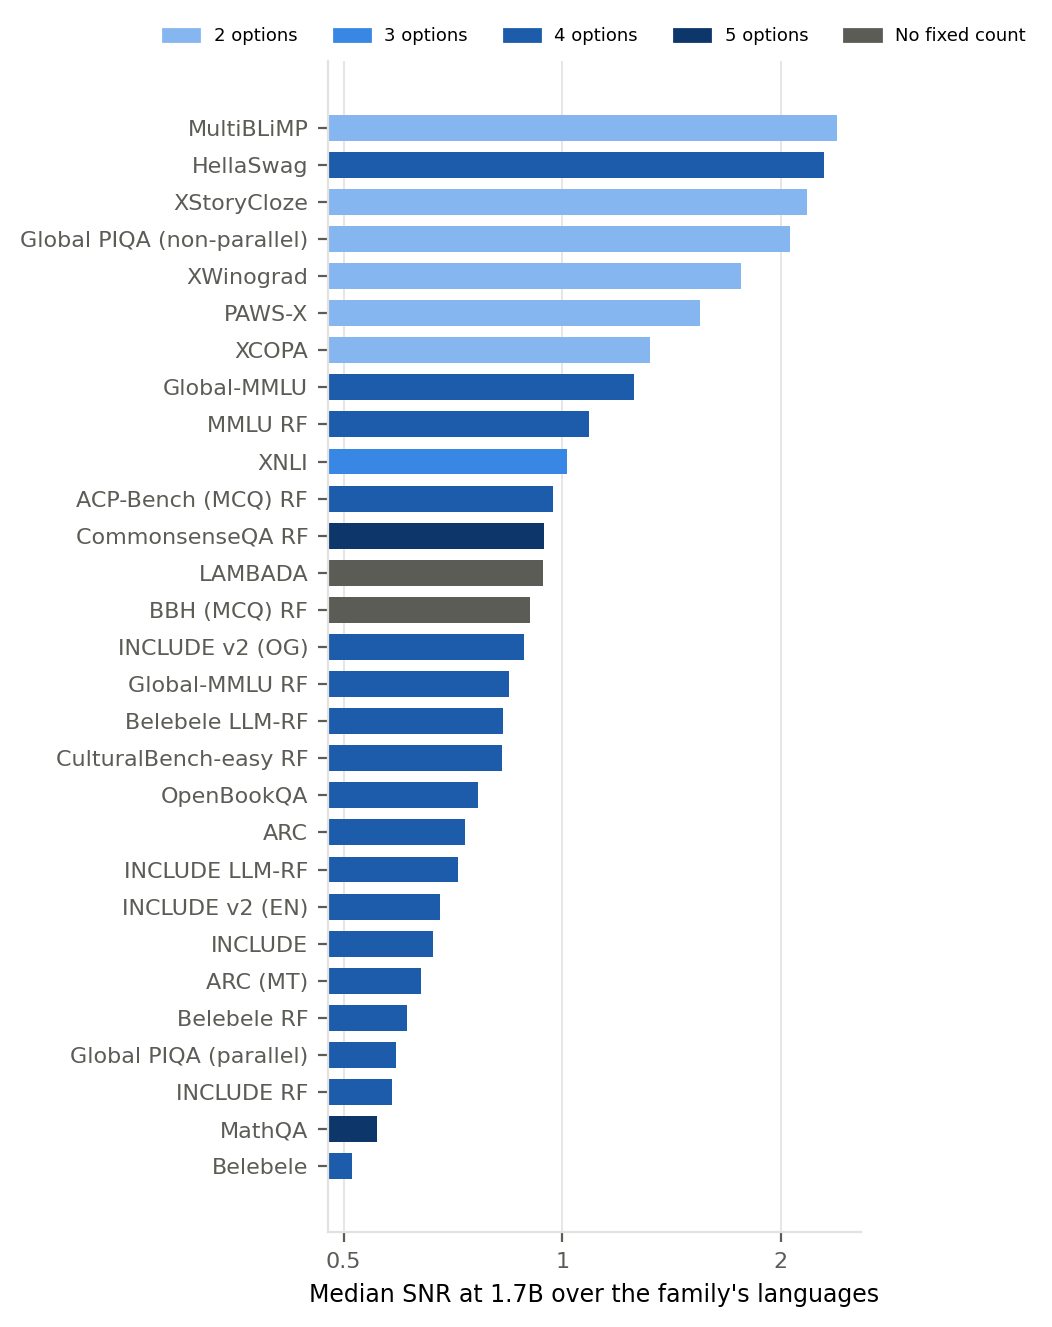
\includegraphics[width=\textwidth,height=0.8\textheight,keepaspectratio]{figures/app_rq09_benchmark_design.png}
% source: src/signal-and-noise/analysis/rq09_benchmark_design/pretraining/predictivity/snr_per_family_ranked_paper.png
\caption{\textbf{With every benchmark in, the answer-option count orders the families by SNR, but no characteristic orders them by DA-size in both readings.} Median SNR at 1.7B over the languages of each benchmark family that clears the above-chance gate, ranked. The colour gives the number of answer options.}
\label{fig:app_rq09_benchmark_design}
\end{figure*}

\begin{table*}[p]
\centering
\small
\caption{\textbf{The 29 benchmark families of the benchmark design analysis and the characteristics it groups them by.} 14 are translated from English, 7 are English originals evaluated in English, and 18 have four answer options. Curation: how the items in each language were made (native: written in the language, English: written in English, human transl.: translated by people, MT: machine translated, MT + post-edit: machine translated and corrected, transl. (unknown): translated by a method the dataset does not document, template: generated from treebank or planning templates). Source: whether the benchmark was translated from English, written natively in several languages or written in English. Format (as the evaluation prompts it): MCQ is a question with lettered options, cloze scores each option as a continuation of the question, completion scores continuations of a context, statement (LLM-RF) is the LLM rewrite into a statement with four continuations, last word scores the final word of a passage. Options gives the range where subtasks differ. Unknown marks a characteristic no source settles, which the analysis leaves out. Context and Option: the median characters of the context and of an option over 100 sampled English items.}
\label{tab:app_rq09_benchmark_characteristics}
\begin{tabular}{lllllrrr}
\toprule
Benchmark & Curation & Source & Format & Options & Passage & Context & Option \\
\midrule
ARC & MT & translated & MCQ & 4 & no & 122 & 28 \\
Belebele & human transl. & translated & MCQ + passage & 4 & yes & 558 & 21 \\
Belebele LLM-RF & human transl. & translated & statement (LLM-RF) & 4 & yes & -- & -- \\
Belebele RF & human transl. & translated & cloze (RF) & 4 & yes & -- & -- \\
Global PIQA (parallel) & native & native & completion & 2 & no & -- & -- \\
Global-MMLU & MT + post-edit & translated & MCQ & 4 & no & 120 & 11 \\
Global-MMLU RF & MT + post-edit & translated & cloze (RF) & 4 & no & -- & -- \\
HellaSwag & MT & translated & completion & 4 & yes & 118 & 61 \\
INCLUDE & native & native & MCQ & 4 & no & -- & -- \\
INCLUDE LLM-RF & native & native & statement (LLM-RF) & 4 & no & -- & -- \\
INCLUDE RF & native & native & cloze (RF) & 4 & no & -- & -- \\
MultiBLiMP & template & native & minimal pair & 2 & no & 46 & 119 \\
PAWS-X & human transl. & translated & classification & 2 & no & 224 & 2 \\
XCOPA & human transl. & translated & completion & 2 & no & 37 & 31 \\
XNLI & human transl. & translated & classification & 3 & no & 127 & 10 \\
XStoryCloze & human transl. & translated & completion & 2 & yes & 189 & 38 \\
XWinograd & native & native & completion & 2 & no & 74 & 6 \\
\bottomrule
\end{tabular}

% source: src/signal-and-noise/analysis/rq09_benchmark_design/pretraining/predictivity/benchmark_characteristics.tex
\end{table*}

\begin{figure*}[p]
\centering
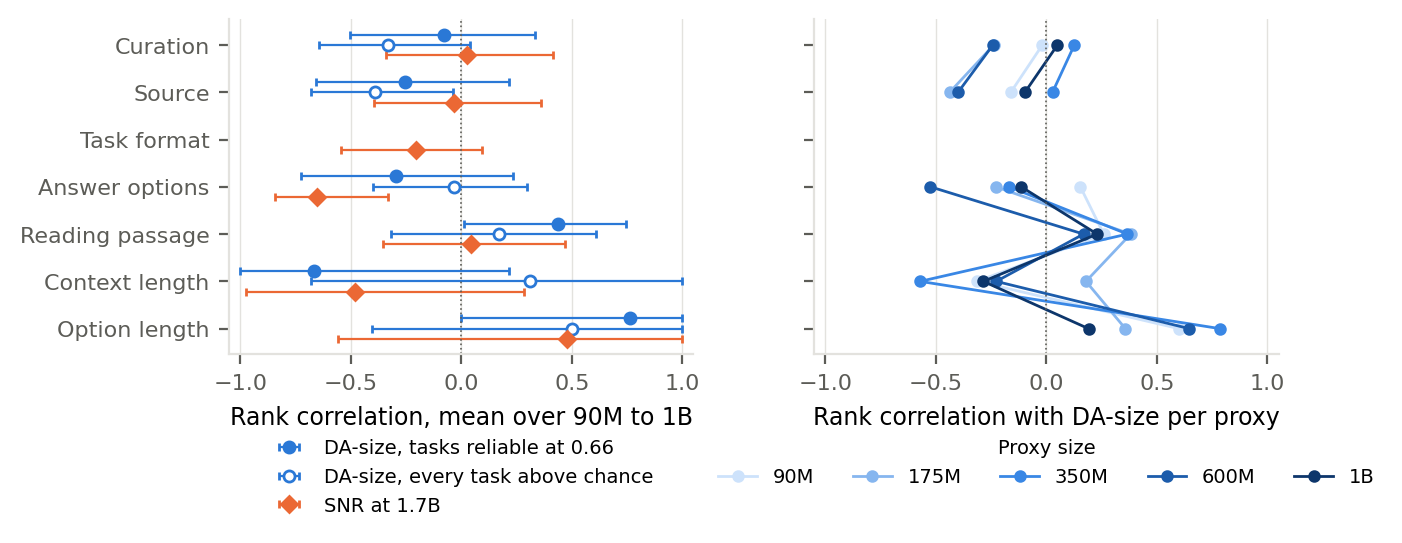
\includegraphics[width=\textwidth,height=0.8\textheight,keepaspectratio]{figures/app_rq09_design_da_correlation.png}
% source: src/signal-and-noise/analysis/rq09_benchmark_design/pretraining/predictivity/design_da_size_correlation_above_66_either_mono_axis_paper.png
\caption{\textbf{No characteristic orders the benchmarks by DA-size in both readings.} The answer options, which correlate with SNR at $\rho = -0.65$ ($-0.84$ to $-0.33$), reach $-0.30$ on the reliable tasks and $-0.03$ on every task above chance. A row is one characteristic of the benchmark families (Table \ref{tab:app_rq09_benchmark_characteristics}). The value is a Spearman $\rho$ over the benchmarks against the characteristic's code: the options ranked 2 to 5, no passage to passage, and the two lengths as they are. Curation, source and task format are split in two: translated to native (written in the language, English originals included, or generated from treebanks or planning problems), translated from English to not, and continuation to lettered options. A split whose smaller side holds one benchmark has no value, so task format has none on DA-size, where INCLUDE is the only benchmark with lettered options. A characteristic marked unknown in the table leaves that benchmark out of its row. DA-size is the per-task DA-size of Figure~\ref{fig:rq2}: the final checkpoint of each proxy against the 1.7B final, on the mono-axis design pairs of the seed-1904 runs, on the tasks above chance at the proxy and at 1.7B. A benchmark's DA-size is the median over its tasks at a proxy, averaged over the proxies 90M--1B. Left: that mean with a 95\% bootstrap interval over the 19 benchmarks whose tasks pass the reliability filter of Figure~\ref{fig:rq2} (filled), over the 27 benchmarks with any task above chance (hollow), and the same statistics on the median SNR at 1.7B of the 29 benchmarks (diamonds). Right: one line per proxy size, on the reliable tasks. The lengths exist for the original benchmarks with sampled items only.}
\label{fig:app_rq09_design_da_correlation}
\end{figure*}

\begin{figure*}[p]
\centering
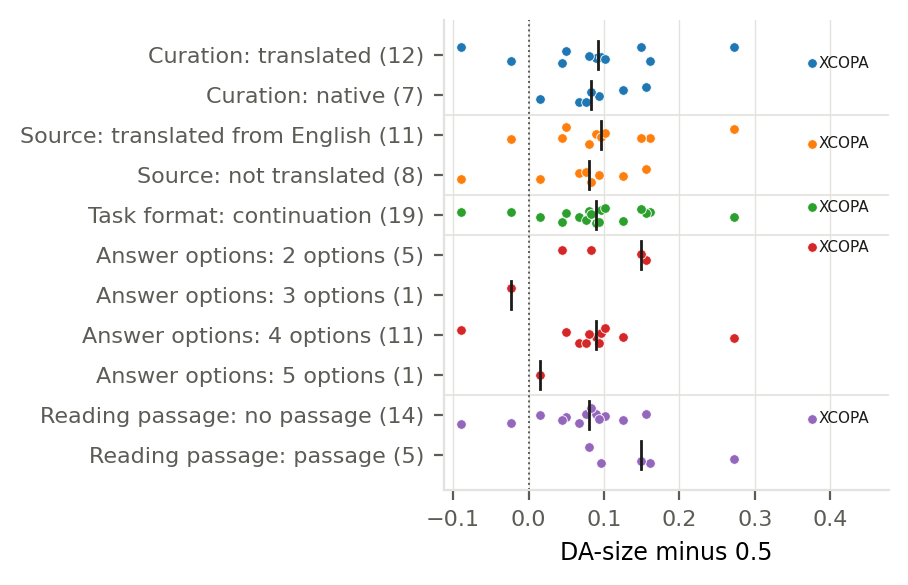
\includegraphics[width=\textwidth,height=0.8\textheight,keepaspectratio]{figures/app_rq09_design_da_by_level.png}
% source: src/signal-and-noise/analysis/rq09_benchmark_design/pretraining/predictivity/design_da_size_by_level_above_66_either_mono_axis_paper.png
\caption{\textbf{XCOPA has the highest DA-size of the 19 benchmarks (0.88), so the levels it carries (translated, translated from English, continuation, 2 options, no passage) are lifted by one benchmark.} Each row is one level of one characteristic, coloured by characteristic, with the number of benchmarks at that level. A dot is one benchmark at its DA-size minus 0.5, so the dotted line is chance agreement, and 17 of the 19 benchmarks sit to its right. The bar is the level's median. DA-size is the per-task DA-size of Figure~\ref{fig:rq2}: the final checkpoint of each proxy against the 1.7B final, on the mono-axis design pairs of the seed-1904 runs, on the tasks above chance at the proxy and at 1.7B. A benchmark's DA-size is the median over its tasks at a proxy, averaged over the proxies 90M--1B, on the tasks that pass the reliability filter of Figure~\ref{fig:rq2}. XCOPA is named on its dot once per characteristic.}
\label{fig:app_rq09_design_da_by_level}
\end{figure*}

\begin{figure*}[p]
\centering
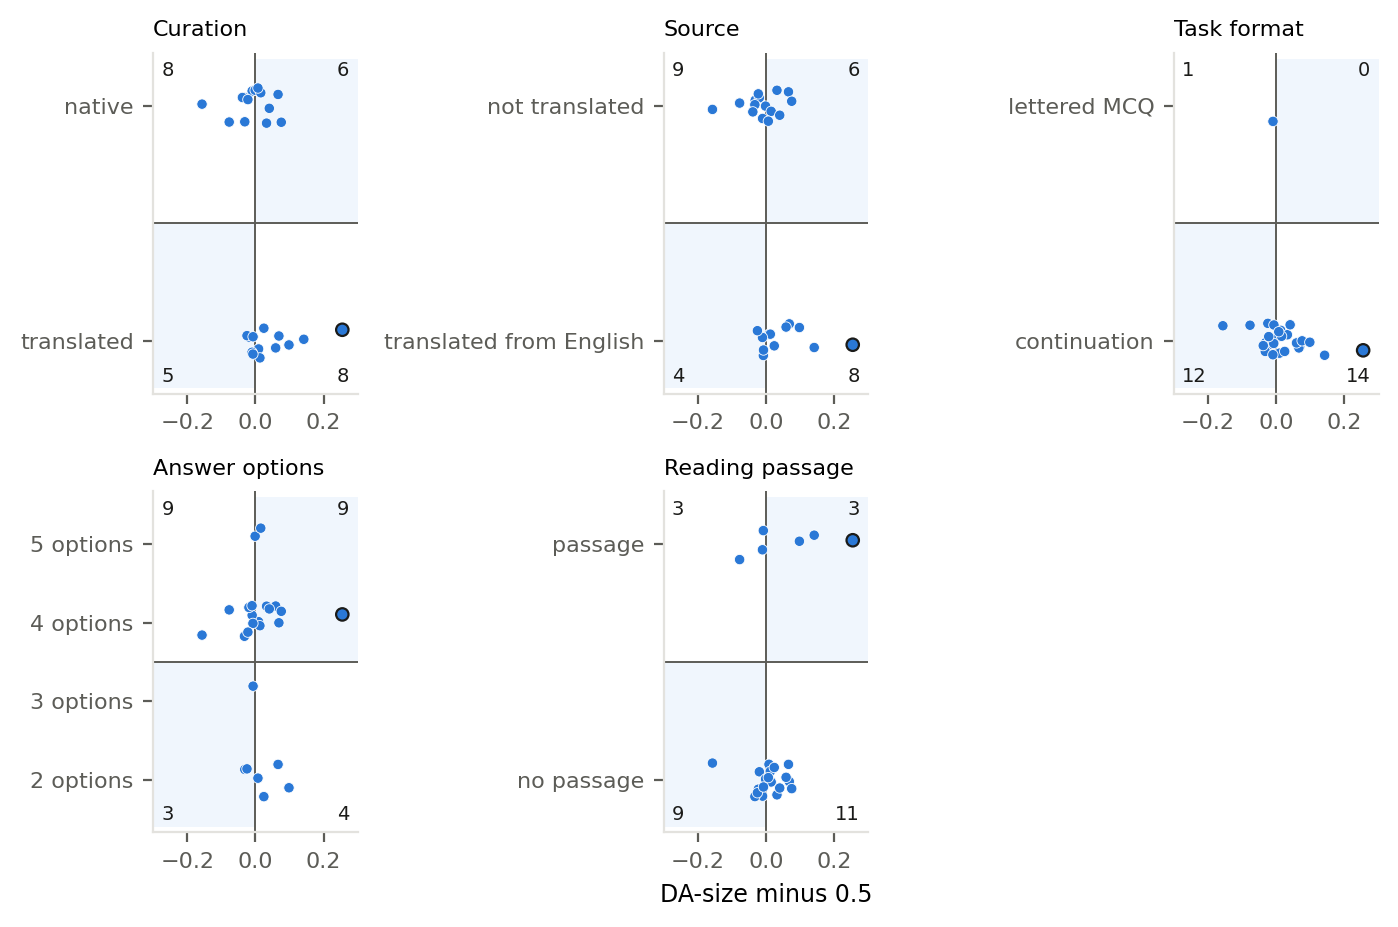
\includegraphics[width=\textwidth,height=0.8\textheight,keepaspectratio]{figures/app_rq09_design_da_quadrant.png}
% source: src/signal-and-noise/analysis/rq09_benchmark_design/pretraining/predictivity/design_da_size_quadrant_mono_axis_paper.png
\caption{\textbf{On every task above chance, 13 of the 27 benchmarks decide below chance agreement (CulturalBench-easy RF, ACP-Bench (MCQ) RF, BBH (MCQ) RF, INCLUDE v2 (OG), Global PIQA (non-parallel), XCOPA, INCLUDE LLM-RF, INCLUDE v2 (EN), Belebele RF, INCLUDE, Belebele LLM-RF, XNLI, MathQA), and they fall on both levels of every characteristic.} One panel per characteristic: x is the DA-size minus 0.5, so the vertical line is chance agreement, and y the characteristic's code centred at 0 (the options ranked 2 to 5 as $-1$, $-1/3$, $+1/3$, $+1$, every other characteristic split in two as $-1$ and $+1$), jittered. The numbers count the benchmarks per quadrant. The shaded quadrants are the ones a positive correlation fills. HellaSwag is outlined. DA-size is the per-task DA-size of Figure~\ref{fig:rq2}: the final checkpoint of each proxy against the 1.7B final, on the mono-axis design pairs of the seed-1904 runs, on the tasks above chance at the proxy and at 1.7B. A benchmark's DA-size is the median over its tasks at a proxy, averaged over the proxies 90M--1B, on every task above chance at the proxy and at 1.7B.}
\label{fig:app_rq09_design_da_quadrant}
\end{figure*}
